\documentclass[UTF8]{ctexbook}
\usepackage{amsmath}
\usepackage{graphicx}
\usepackage[a4paper,scale=0.8,centering]{geometry}
\begin{document}
	\chapter{机器学习}
	\section{机器学习简介}
人工智能是我们想要达到的目标,机器学习则是实现人工智能的手段,深度学习则是机器学习的其中一种。

那么机器学习是什么? 机器学习可以看做是从数据中学习一个函数 (function),对于给定输入得到输出结果。如在语音辨识、图像识别等领域的应用。

机器学习框架如图 \ref{fig:ml_framework} 所示,首先包含一系列函数 model 的集合,利用训练数据评价函数的品质,并挑选出最优函数模型。

\begin{figure}[ht]
	\centering
	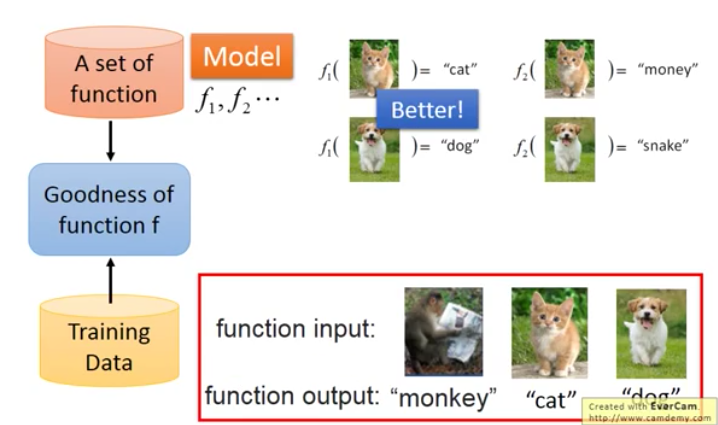
\includegraphics[scale=0.4]{./pic/ml_framework.png}
	\caption{机器学习框架}
	\label{fig:ml_framework}
\end{figure}
  
详细步骤如图 \ref{fig:three_step} 所示,可以总结为:

\begin{enumerate}
	\item 挑选模型
	\item 评价函数品质 goodness
	\item 挑选最优函数 $f^*$
\end{enumerate}
	
\begin{figure}[ht]
	\centering
	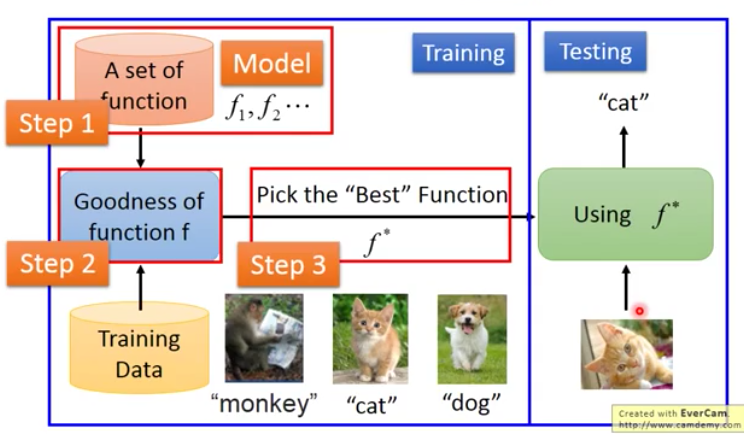
\includegraphics[scale=0.4]{./pic/three_step_of_ml.png}
	\caption{机器学习三步骤}
	\label{fig:three_step}
\end{figure}

机器学习的学习图谱如图 \ref{fig:ml_map} 所示,具体描述如下:

\begin{figure}[ht]
	\centering
	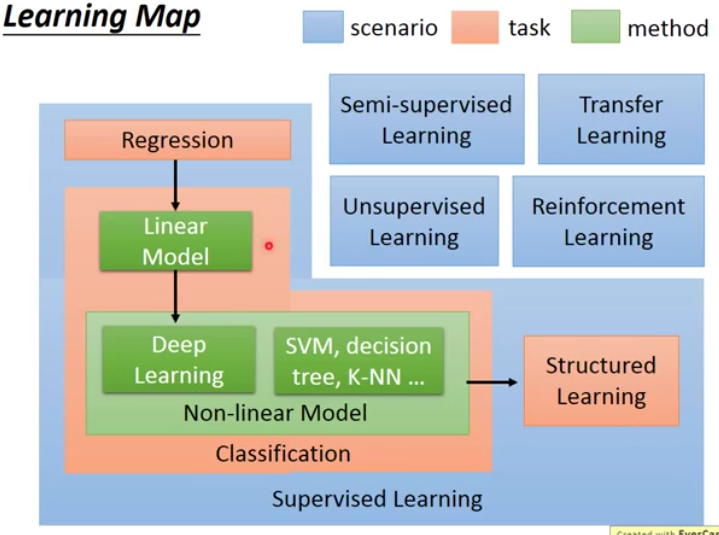
\includegraphics[scale=0.4]{./pic/learning_map.png}
	\caption{机器学习图谱}
	\label{fig:ml_map}
\end{figure}
	
\begin{enumerate}
	\item 监督学习
		\subitem 回归
		\subitem 线性模型
		\subitem 深度学习,非线性模型
		\subitem 其它非线性模型,如SVM、决策树、knn。
		\subitem structure learning
	\item 无监督学习
	\item 半监督学习
	\item 迁移学习
	\item 强化学习

\end{enumerate}

\section{回归问题}
线性模型:$y=b+\sum w_i x_i$,其中$x_i$ 为输入数据的特征,$w_i$为权重,$b$为偏置。

使用损失函数评价选定模型的好坏。如对于模型$f$,样本$x^n$,对应的输出真值为$\hat{y}$:
\[
	L(f)=\sum_{n=1}^{N}\left( \hat{y}^n - f(x_{cp}^n) \right)^2
\]
对于线性模型:
\[
	L(w,b)=\sum_{n=1}^{N}\left( \hat{y}^n - (b+w \cdot x_{xp}^n) \right)^2
\]
最优化模型:
\[
	w ^ { * } , b ^ { * } = \arg \min _ { w , b } L ( w , b )= \arg \min _ { w , b } \sum _ { n = 1 } ^ { N } \left( \hat { y } ^ { n } - ( b + w \cdot x _ { c p } ^ { n } ) \right) ^ { 2 }
\]
\end{document}